%UML und Shit

%Subfile of pflichtenheft
\documentclass[../pflichtenheft.tex]{subfiles}

%New Command for hyperlinks
\newcommand{\gt}[1]{\hyperlink{t#1}{/T#1/}}
\newcommand{\fa}[1]{\falink{#1}}
\newcommand{\view}[1]{\hypertarget{v#1}{/V#1/}}

\begin{document}

%need to add/update references to gt
\vspace{100pt}
\section{Systemmodelle}
	\subsection{Szenarien}

		\subsubsection{Verbinden der Earables}
		\label{sec:verbindenS}
			\begin{enumerate}
				\item \gt{701} App öffnen
				\item \gt{301} Nach verfügbaren Bluetooth-Geräten suchen (\fa{302})
				\item \gt{303} Verfügbare Bluetooth-Geräte auflisten (\fa{303})
				\item \gt{302} Suche nach verfügbaren Bluetooth-Geräten aktualisieren (\fa{304})
				\item \gt{303} Verfügbare Bluetooth-Geräte auflisten (\fa{303})
				\item \gt{304} BLE- und BC-Verbindung zu den Earables herstellen (\fa{305})
				\item \gt{305} BLE- und BC-Verbindung zu den Earables trennen (\fa{306})
				\item \gt{702} App schließen
			\end{enumerate}
			\hyperref[sec:verbinden]{UML-Aktivitäts-Diagramm}
		\subsubsection{Verwaltung der Audio-Bibliothek 1}
		\label{sec:verwaltung1S}
			\begin{enumerate}
				\item \gt{701} App öffnen
				%\item \gt{301} Nach verfügbaren Bluetooth-Geräten suchen (\fa{302})
				%\item \gt{303} Verfügbare Bluetooth-Geräte auflisten (\fa{303})
				%\item \gt{304} BLE- und BC-Verbindung zu den Earables herstellen (\fa{305})
				\item \gt{401} Audio-Bibliothek öffnen (\fa{320})
				\item \gt{402} Audio-Datei der Bibliothek hinzufügen (\fa{321}, \fa{322})
				\item \gt{403} Metadaten einer Audio-Datei auslesen (\fa{323})
				\item \gt{404} Metadaten einer Audio-Datei manuell bearbeiten (\fa{324})
				\item \gt{411} Audio-Bibliothek durchsuchen nach Titel (\fa{326})
				\item \gt{412} Audio-Bibliothek durchsuchen nach Künstler (\fa{326})
				\item \gt{405} Audio-Datei aus der Bibliothek löschen (\fa{325})
				\item \gt{418} Audio-Bibliothek schließen (\fa{320})
				\item \gt{702} App schließen
			\end{enumerate}
			\hyperref[sec:verwaltung1]{UML-Aktivitäts-Diagramm}
		\subsubsection{Verwaltung der Audio-Bibliothek 2}
		\label{sec:verwaltung2S}
			\begin{enumerate}
				\item \gt{701} App öffnen
				%\item \gt{301} Nach verfügbaren Bluetooth-Geräten suchen (\fa{302})
				%\item \gt{303} Verfügbare Bluetooth-Geräte auflisten (\fa{303})
				%\item \gt{304} BLE- und BC-Verbindung zu den Earables herstellen (\fa{305})
				\item \gt{401} Audio-Bibliothek öffnen (\fa{320})
				\item \gt{402} Audio-Datei der Bibliothek hinzufügen (\fa{321}, \fa{322})
				\item \gt{403} Metadaten einer Audio-Datei auslesen (\fa{323})
				\item \gt{404} Metadaten einer Audio-Datei manuell bearbeiten (\fa{324})
				\item Schritte 3. - 5. wiederholen
				\item \gt{414} Audio-Bibliothek nach Titel sortieren (\fa{327})
				\item \gt{415} Audio-Bibliothek nach Künstler sortieren (\fa{327})
				%\item \gt{903} Es muss mindestens ein Lied in der Audiobibliothek vorhanden bevor
				%diese automatisch bezuglich eines BPM-Wert durchsucht werden kann
				\item \gt{416} Audio-Bibliothek nach BPM-Wert sortieren (\fa{327})
				\item \gt{418} Audio-Bibliothek schließen (\fa{320})
				\item \gt{702} App schließen
			\end{enumerate}
			\hyperref[sec:verwaltung2]{UML-Aktivitäts-Diagramm}
		\subsubsection{Abspielfunktionen von Audio-Dateien}
		\label{sec:abspielenS}
			\begin{enumerate}
				\item \gt{701} App öffnen
				\item Bluetooth Verbindung herstellen [\gt{301},\gt{303},\gt{304}]
				\item \gt{401} Audio-Bibliothek öffnen (\fa{320})
				\item \gt{402} Audio-Datei der Bibliothek hinzufügen (\fa{321}, \fa{322})
				\item \gt{403} Metadaten einer Audio-Datei auslesen (\fa{323})
				\item \gt{404} Metadaten einer Audio-Datei manuell bearbeiten (\fa{324})
				\item Schritte 4. - 6. wiederholen
				\item \gt{406} Audio-Datei auswählen und abspielen über Earables-Output (\fa{330}, \fa{331}, \fa{332})
				\item \gt{407} Audio pausieren bzw. wiedergeben (\fa{333})
         		\item \gt{408} Nächste Audio-Datei in Audio-Bibliothek abspielen (\fa{334})
				\item \gt{409} Vorherige Audio-Datei in Audio-Bibliothek abspielen (\fa{334})
				\item \gt{808} Im Audio-Player die Lautstärke verändern (\falink{336W})
				\item \gt{809} Im Audio-Player den Abspielzeitpunkt verändern (\falink{337W})
				\item \gt{418} Audio-Bibliothek schließen (\fa{320}
				\item \gt{702} App schließen
			\end{enumerate}
			\hyperref[sec:abspielen]{UML-Aktivitäts-Diagramm}
		\subsubsection{Motivationsmusik beim Laufen}
		\label{sec:motivationS}
			\begin{enumerate}
				\item \gt{701} App öffnen
				\item Bluetooth Verbindung herstellen [\gt{301},\gt{303},\gt{304}]
				\item \gt{401} Audio-Bibliothek öffnen (\fa{320})
				\item Audio-Dateien hinzufügen (\gt{402}, \gt{403} und \gt{404} wiederholen)
				\item \gt{801} BPM-Wert einer Audio-Datei berechnen und gespeicherten BPM-Wert überschreiben\footnote{Nur wenn das Wunschkriterium \fa{370W} implementiert wird.}
				\item \gt{418} Audio-Bibliothek schließen (\fa{320})
				\item \gt{601} Modus-Manager öffnen (\fa{340})
				\item \gt{602} Motivationsmusik-Modus anschalten (\fa{341})
				\item \gt{604} Aus Schrittfrequenz passenden BPM-Wert berechnen (\fa{342})
				\item \gt{417} Audio-Datei in Bibliothek finden, deren BPM-Wert am ehesten mit einem gegeben Wert übereinstimmt (\fa{343})
				\item \gt{406} Audio-Datei auswählen und abspielen über Earables-Output (\fa{330}, \fa{331}, \fa{332})
				\item \gt{603} Motivationsmusik-Modus ausschalten (\fa{341})
				\item \gt{605} Modus-Manager schließen (\fa{340})
				\item \gt{702} App schließen
			\end{enumerate}
			\hyperref[sec:motivation]{UML-Aktivitäts-Diagramm}
		\subsubsection{Autostop-Modus beim Laufen}
		\label{sec:autostopS}
			Dieses Szenario gehört zum Wunschkriterium Autostop-Modus \falink{344W}.
			\begin{enumerate}
				\item \gt{701} App öffnen
				%\item \gt{901} Solange die Earables nicht verbunden sind sollen keine Abfragen an die Kopfhörer gestellt werden können
				\item Bluetooth Verbindung herstellen [\gt{301},\gt{303},\gt{304}]
				\item \gt{601} Modus-Manager öffnen (\fa{340})
				\item \gt{802} Autostop-Modus anschalten
				\item \gt{406} Audio-Datei auswählen und abspielen über Earables-Output (\fa{330}, \fa{331}, \fa{332})
				\item \gt{804} Autostop-Modus pausiert Musik wenn nicht in Bewegung
				\item \gt{803} Autostop-Modus ausschalten
				\item \gt{702} App schließen
			\end{enumerate}
			\hyperref[sec:autostop]{UML-Aktivitäts-Diagramm}
		\subsubsection{Konfiguration der Einstellungen}
		\label{sec:konfigS}
			\begin{enumerate}
				\item \gt{701} App öffnen
				\item Bluetooth Verbindung herstellen [\gt{301},\gt{303},\gt{304}]
				\item \gt{501} Einstellungen öffnen (\fa{310})
				\item \gt{502} Sprache ändern (\fa{311})
				\item \gt{806} Geräte-Name der Earables ändern (\fa{312W})
				\item \gt{503} Schrittanzahl zurücksetzen (\fa{354})
				\item \gt{504} Einstellungen schließen (\fa{310})
				\item \gt{702} App schließen
			\end{enumerate}
			\hyperref[sec:konfig]{UML-Aktivitäts-Diagramm}
		\subsubsection{App im Hintergrund laufen lassen}
		\label{sec:hintergrundS}
			\begin{enumerate}
				\item \gt{701} App öffnen
				\item Bluetooth Verbindung herstellen [\gt{301},\gt{303},\gt{304}]
				\item \gt{501} Einstellungen öffnen (\fa{310})
				\item \gt{703} Bildschirm drehen
				\item \gt{703} Bildschirm (zurück) drehen
				\item \gt{504} Einstellungen schließen (\fa{310})
				\item \gt{704} Bildschirm ausschalten
				\item \gt{704} Bildschirm anschalten
				\item \gt{702} App schließen
			\end{enumerate}
			\hyperref[sec:hintergrund]{UML-Aktivitäts-Diagramm}
		\subsubsection{Spotify einbinden}
		\label{sec:spotifyS}
			Dieses Szenario gehört zum Wunschkriterium Spotify-Unterstützung \fa{360W}.
			\begin{enumerate}
				\item \gt{701} App öffnen
				\item Bluetooth Verbindung herstellen [\gt{301},\gt{303},\gt{304}]
				\item \gt{804} App mit Spotify-Account verbinden
				\item \gt{805} Modi des Modus-Managers in Kombination mit der persönlichen Spotify-Bibliothek anstelle der integrierten Audio-Bibliothek nutzen
				\item \gt{401} Audio-Bibliothek öffnen (\fa{320})
				\item \gt{406} Audio-Datei auswählen und abspielen über Earables-Output (\fa{330}, \fa{331}, \fa{332})
				\item \gt{407} Audio pausieren bzw. wiedergeben (\fa{333})
         		\item \gt{408} Nächste Audio-Datei in Audio-Bibliothek abspielen (\fa{334})
				\item \gt{409} Vorherige Audio-Datei in Audio-Bibliothek abspielen (\fa{334})
				\item \gt{401} Audio-Bibliothek schließen (\fa{320})
				\item \gt{702} App schließen
			\end{enumerate}
			\hyperref[sec:spotify]{UML-Aktivitäts-Diagramm}
	%\subsection{Anwendungsfälle}
		%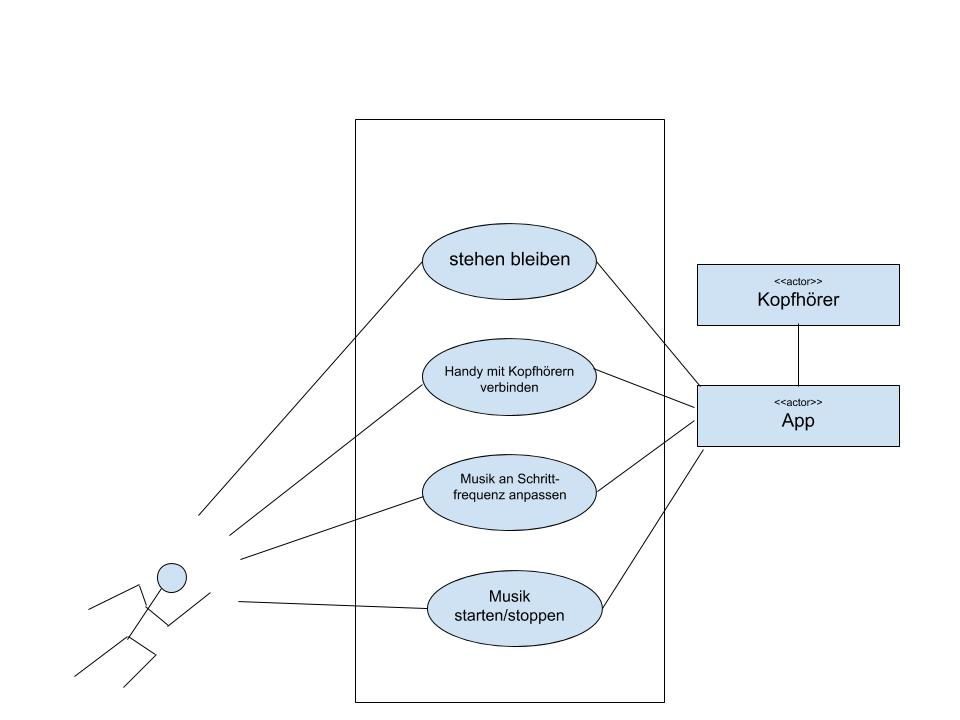
\includegraphics[page=1,width=400pt,keepaspectratio]{../graphics/UML/eSense_Anwendungsfall.jpg}
	\subsection{Architekturmodell}
		\vspace{10mm}
		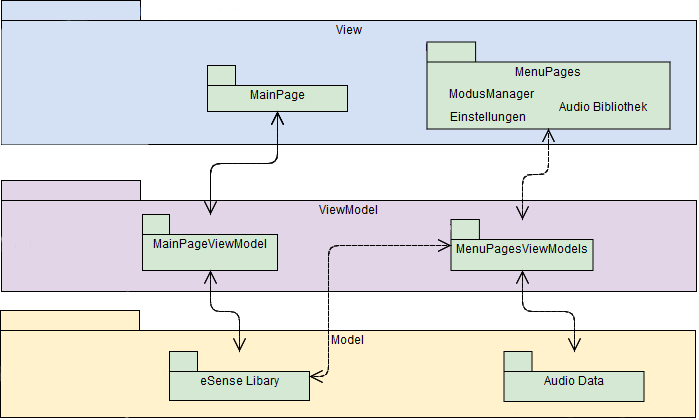
\includegraphics[page=1,width=400pt,keepaspectratio]{../graphics/UML/eSensePackageDiagram.png}
		\begin{center}
			\textit{Model-View-Viewmodel Architektur der App (Komponente 3)}
		\end{center}
		\subsection{Dynamische Modelle}
		\subsubsection{Verbinden der Earables}
		\label{sec:verbinden}
			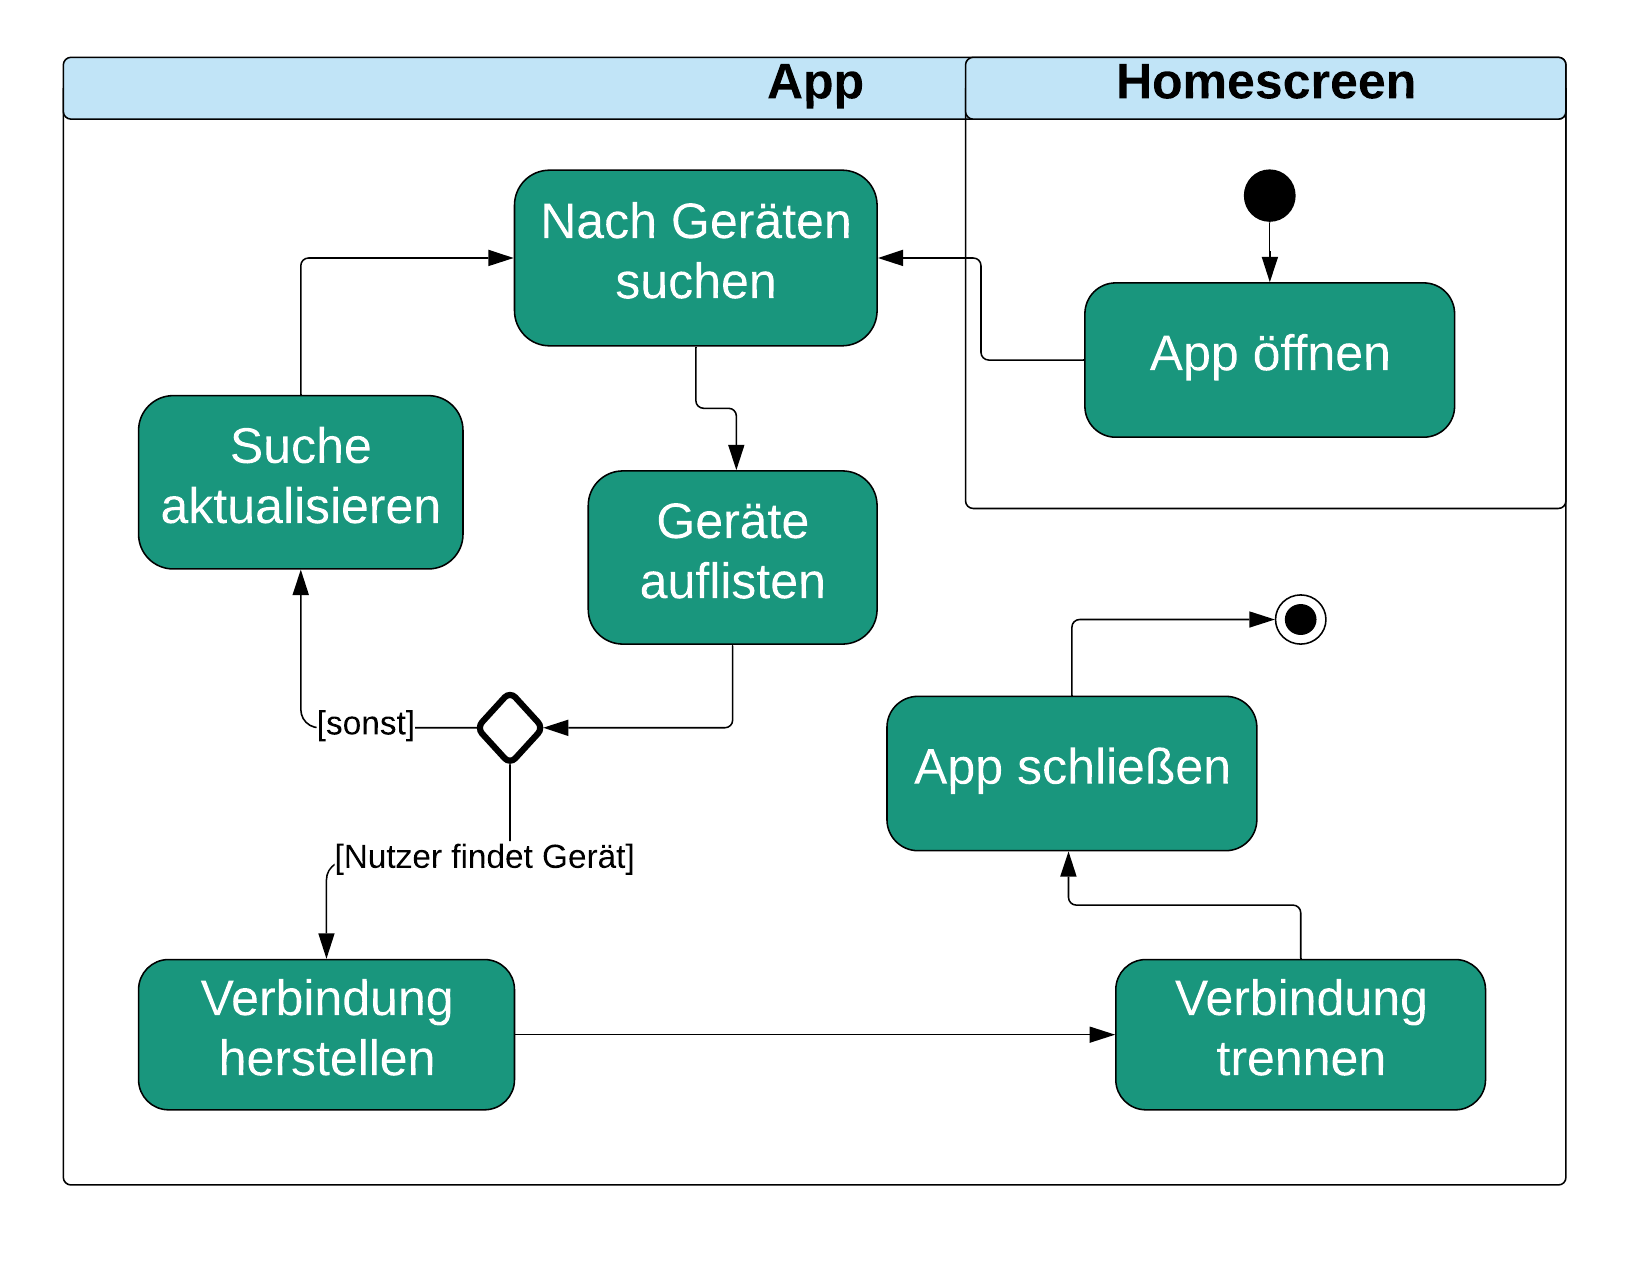
\includegraphics[page=1,width=400pt,keepaspectratio]{../graphics/UML/Verbinden_der_Earables.png}
			Hier testet der \Gls{user} den Verbindungsaufbau mit den \Gls{earable}s (\hyperref[sec:verbindenS]{Szenario})
		\subsubsection{Verwaltung der Audiobibliothek 1}
		\label{sec:verwaltung1}
			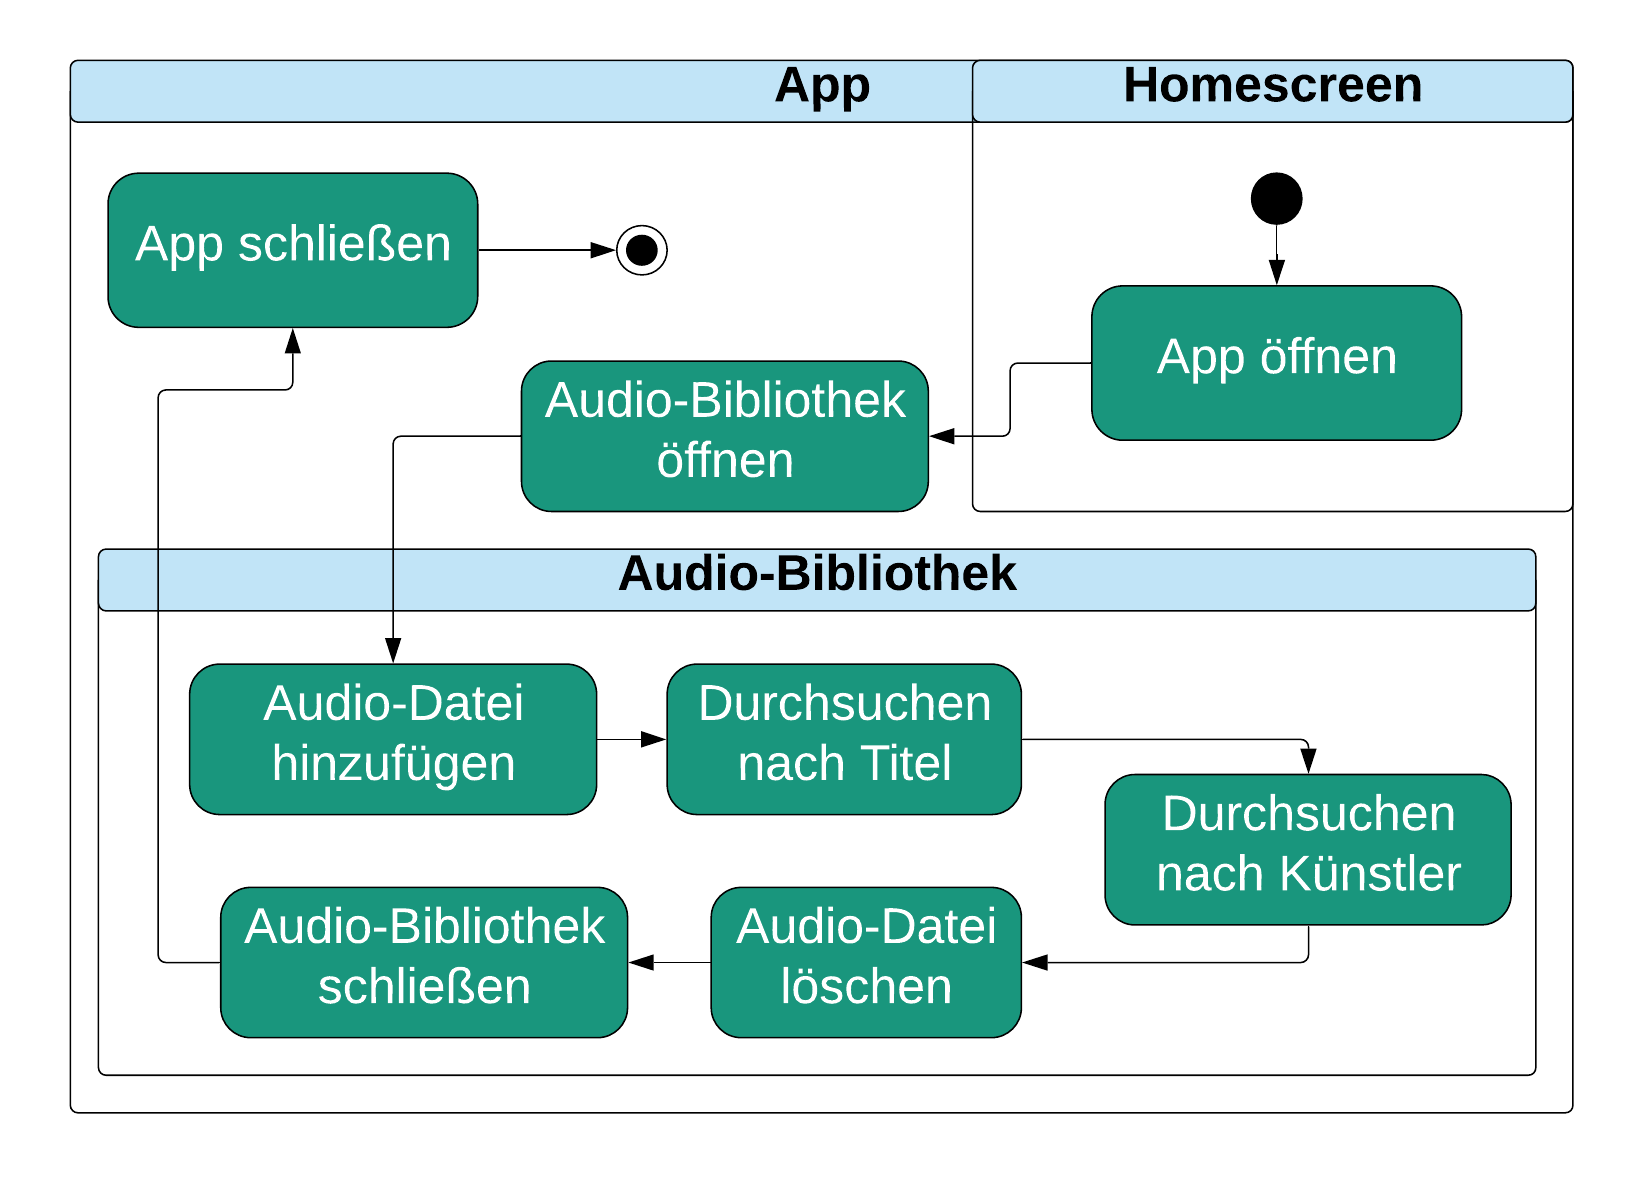
\includegraphics[page=1,width=400pt,keepaspectratio]{../graphics/UML/Verwaltung_der_Audio-Bibliothek_1.png}
			Hier testet der \Gls{user} die Durchsuchungsfunktionen der \Gls{audiolib} (\hyperref[sec:verwaltung1S]{Szenario})
		\subsubsection{Verwaltung der Audiobibliothek 2}
		\label{sec:verwaltung2}
			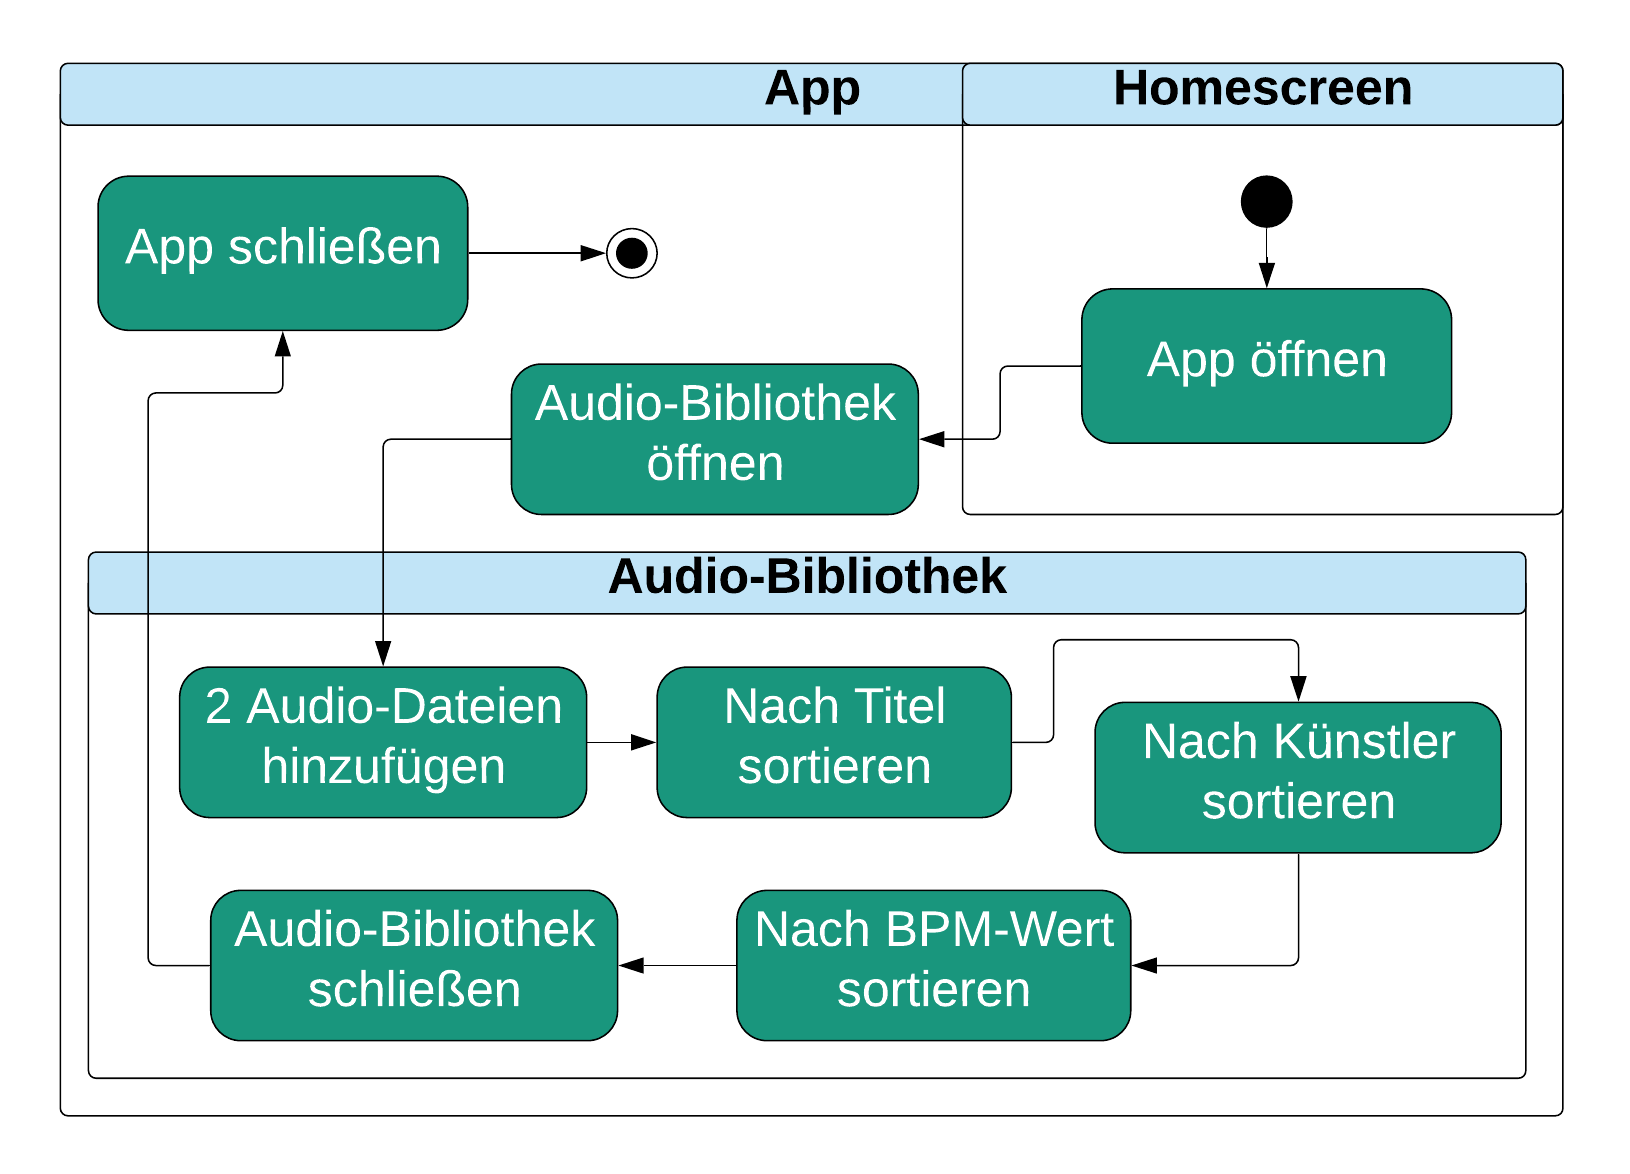
\includegraphics[page=1,width=400pt,keepaspectratio]{../graphics/UML/Verwaltung_der_Audio-Bibliothek_2.png}
			Hier testet der \Gls{user} die Sortierfunktionen der \Gls{audiolib} (\hyperref[sec:verwaltung2S]{Szenario})
		\subsubsection{Abspielfunktionen von Audiodateien}
		\label{sec:abspielen}
			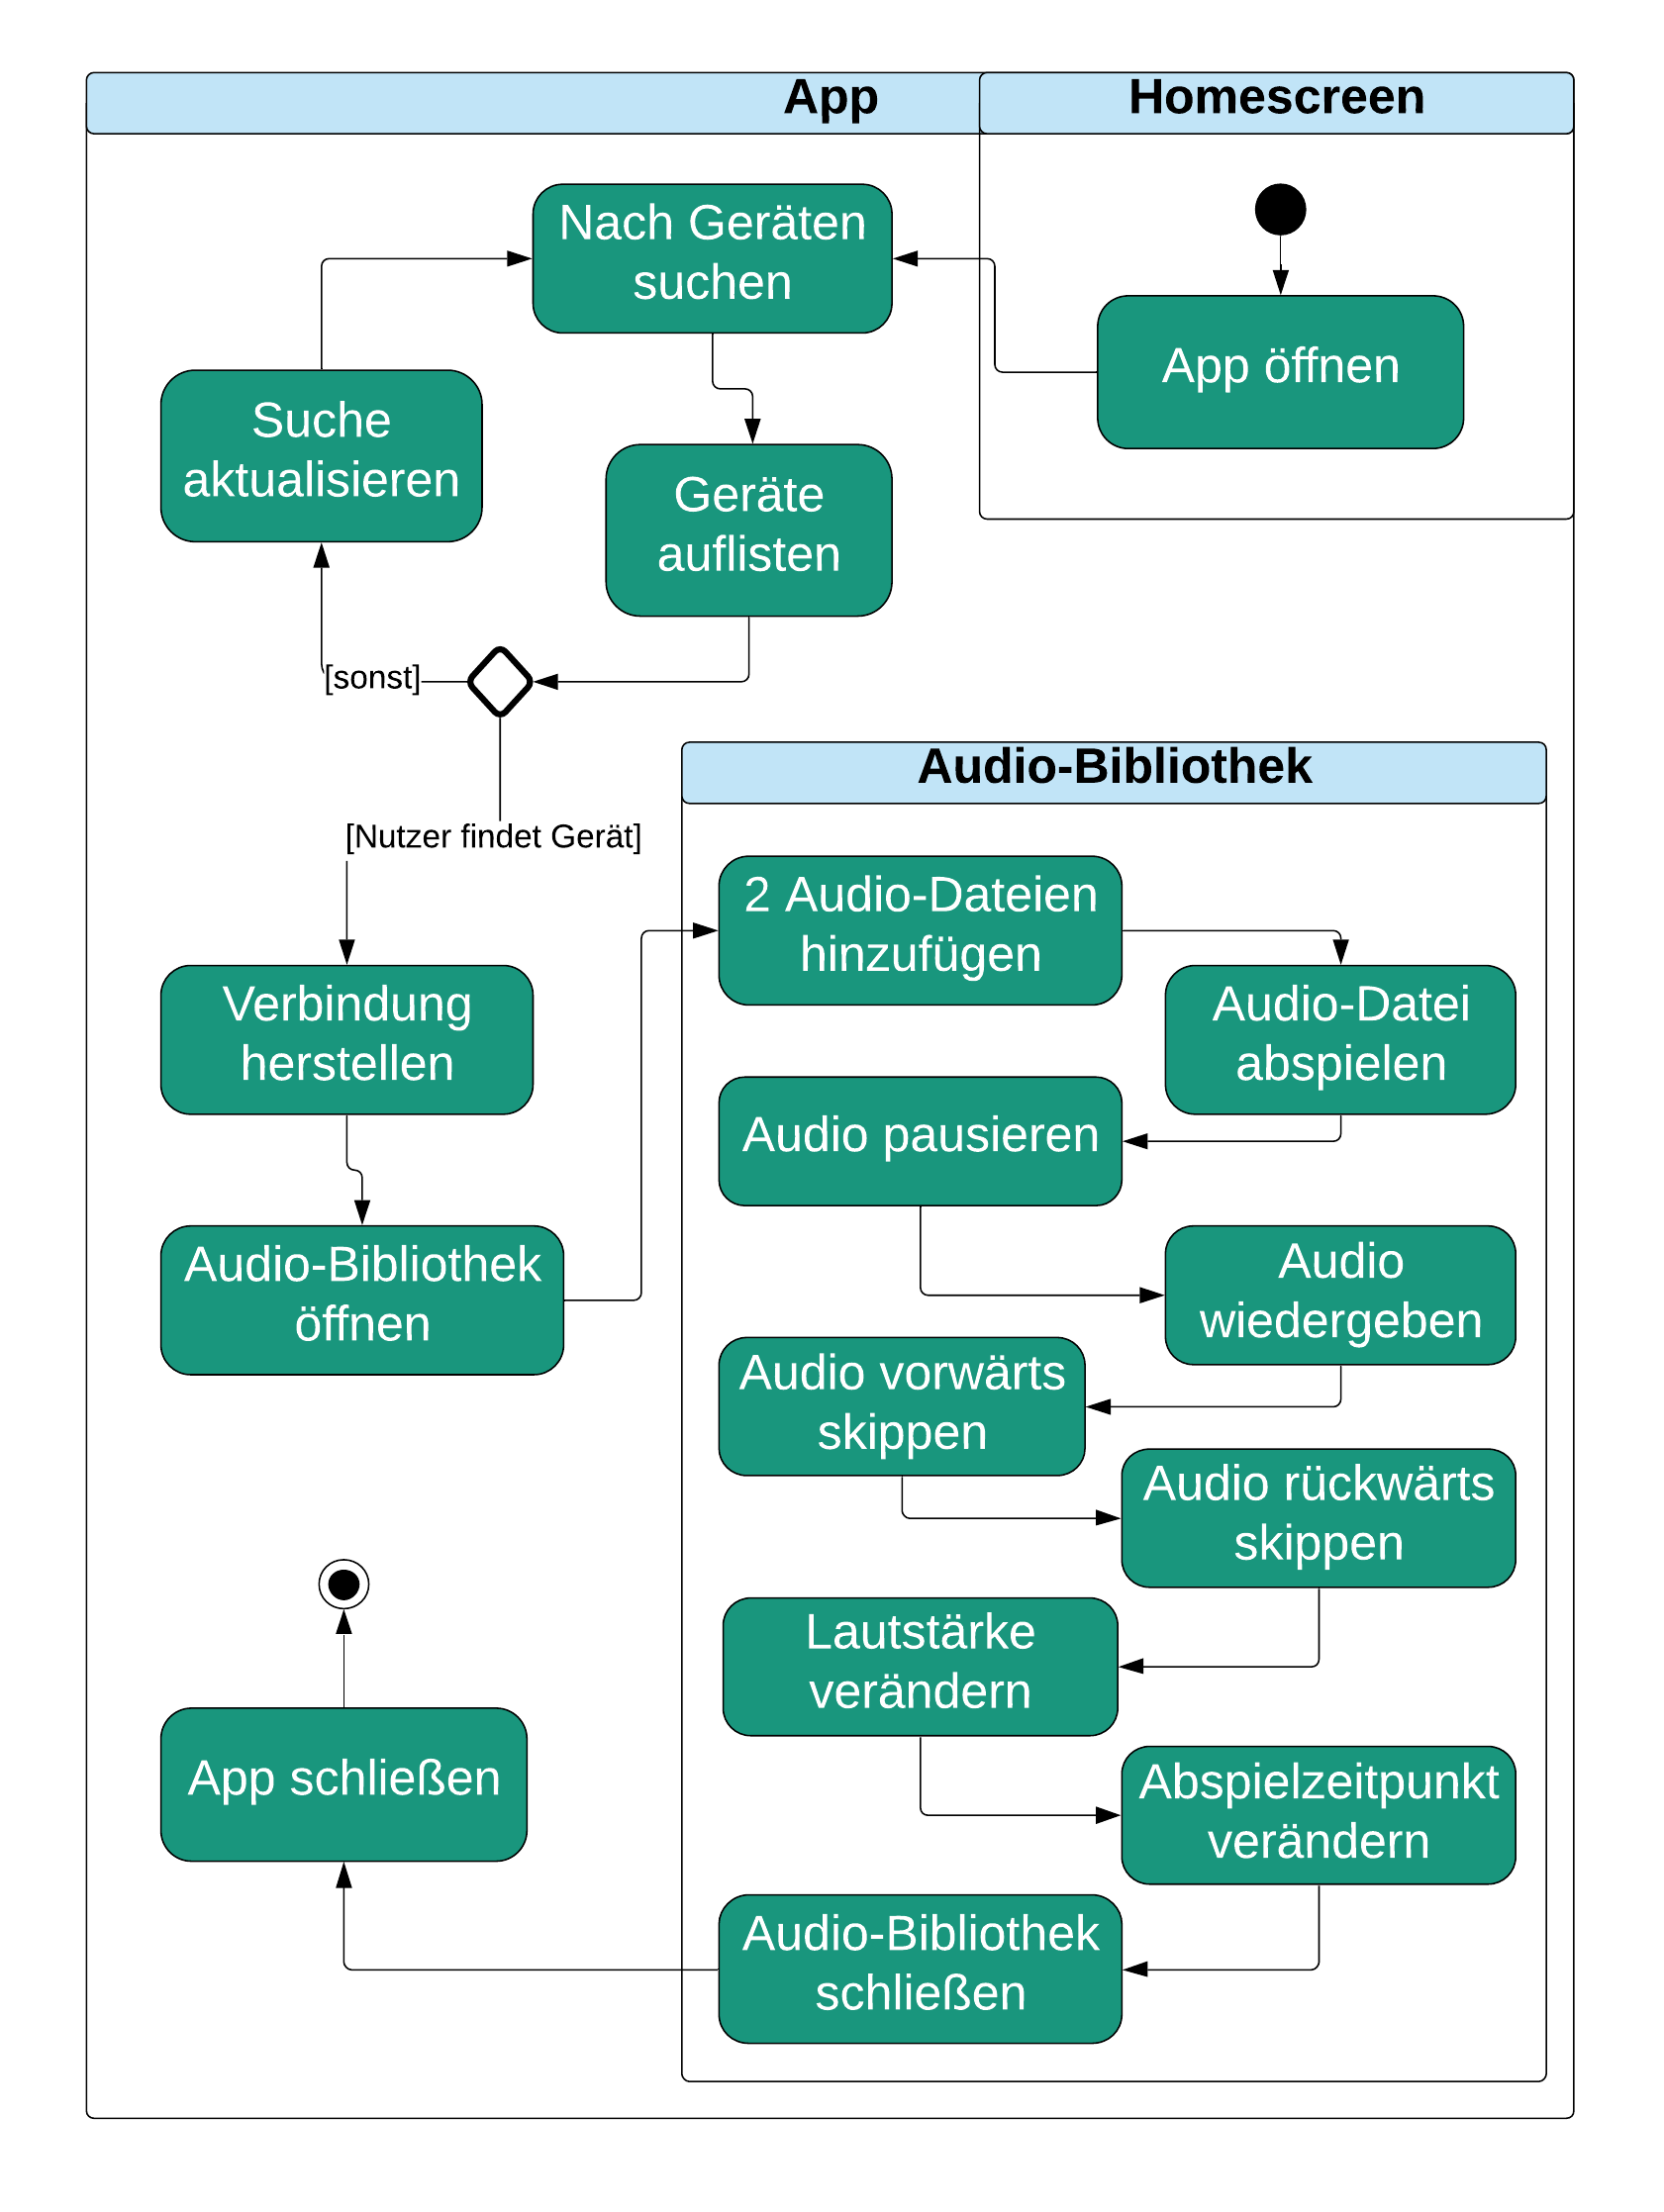
\includegraphics[page=1,width=400pt,keepaspectratio]{../graphics/UML/Abspielfunktionen_von_Audio-Dateien.png}
			Hier testet der \Gls{user} die Funktionen des Audio-Players (\hyperref[sec:abspielenS]{Szenario})
		\subsubsection{Motivationsmusik beim Laufen}
		\label{sec:motivation}
			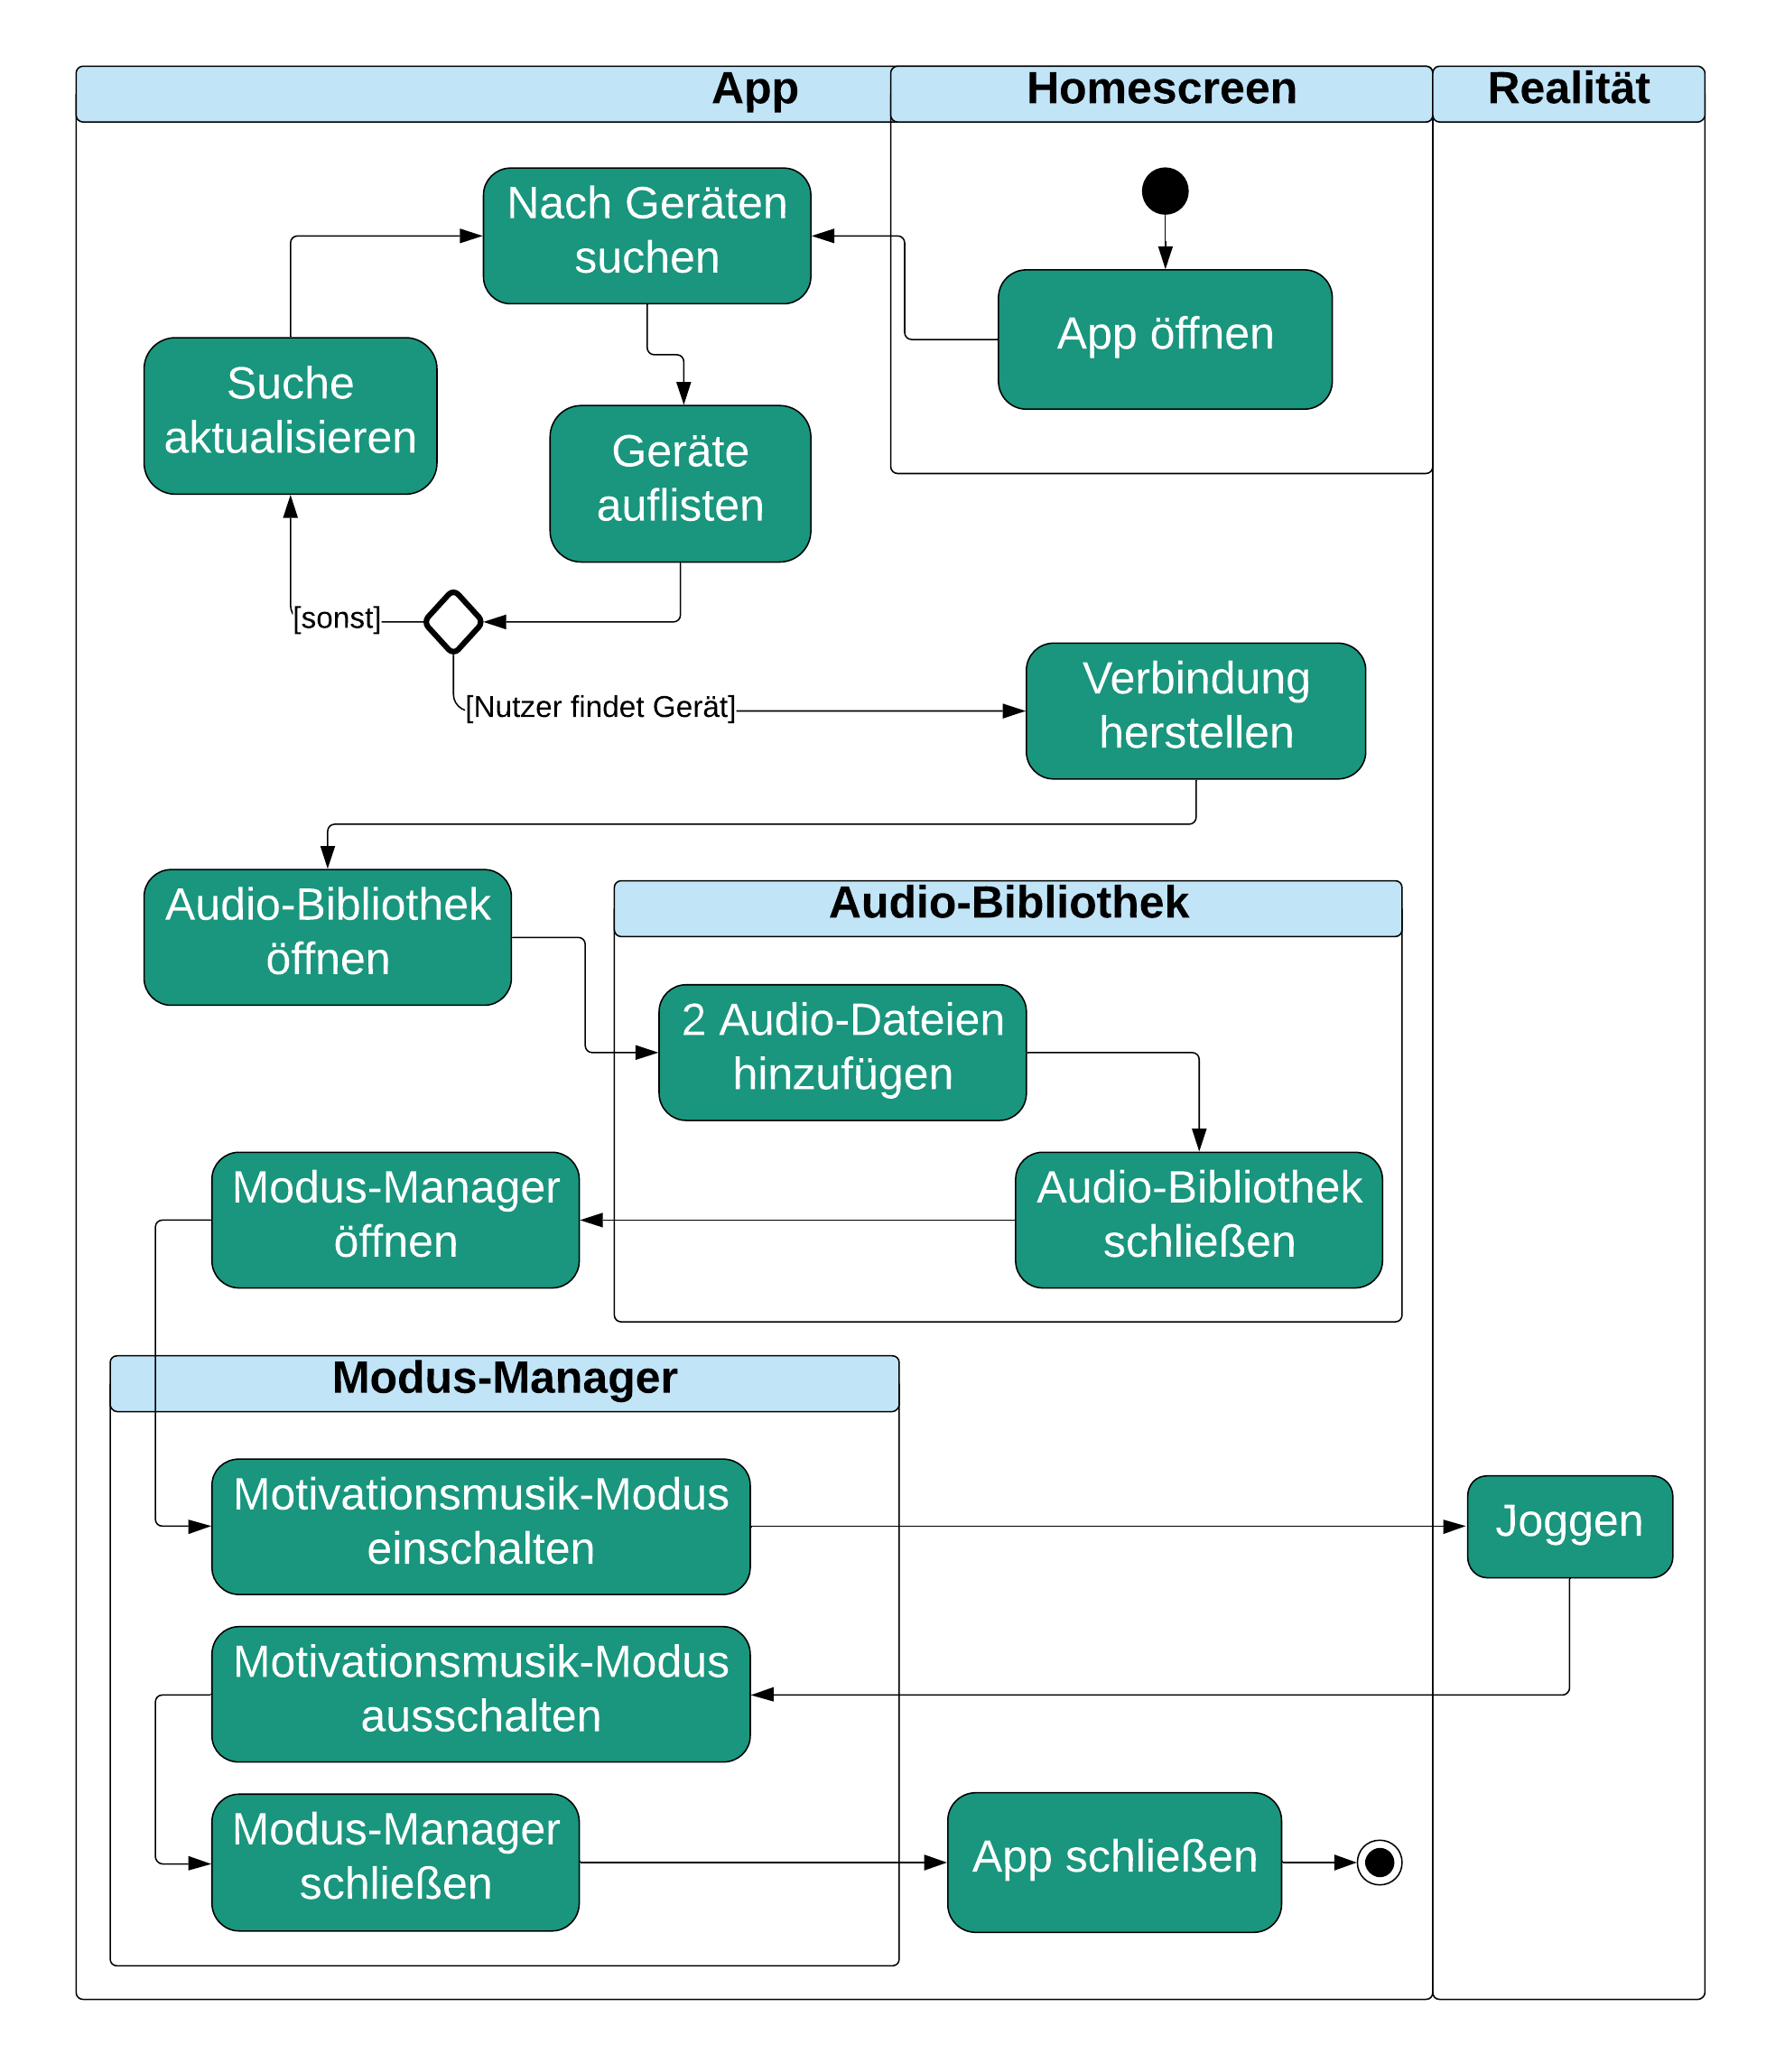
\includegraphics[page=1,width=400pt,keepaspectratio]{../graphics/UML/Motivationsmusik_beim_Laufen.png}
			Hier testet der \Gls{user} den Motivationsmusik-Modus (\hyperref[sec:motivationS]{Szenario})
		\subsubsection{Autostop-Modus beim Laufen}
		\label{sec:autostop}
			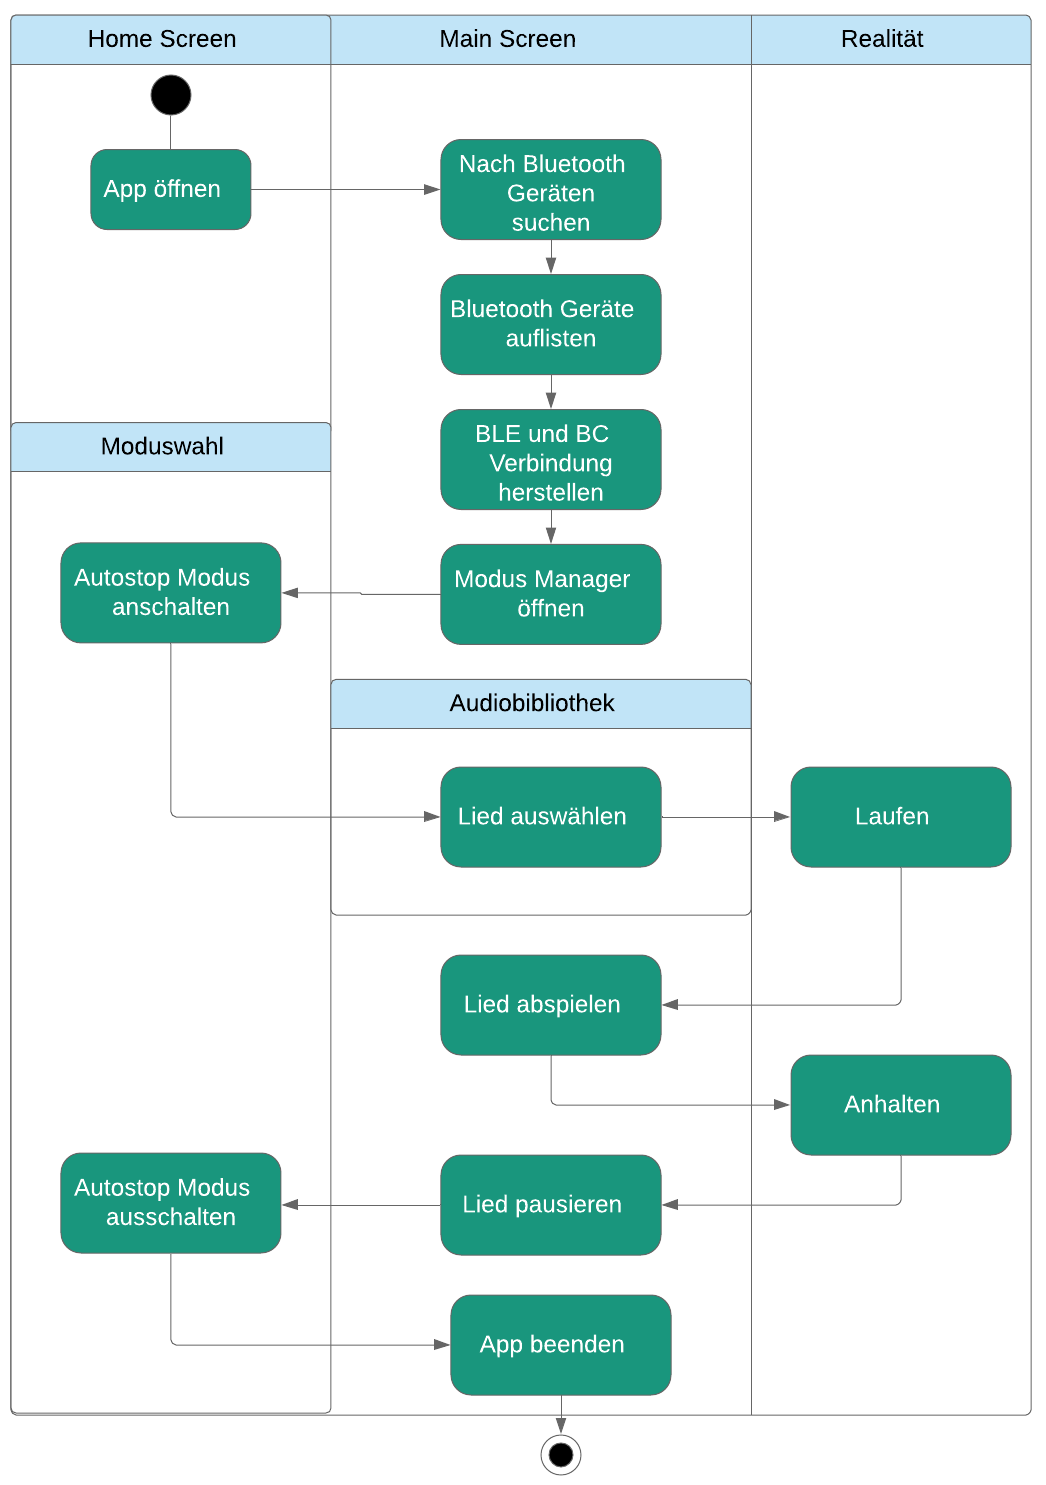
\includegraphics[page=1,width=350pt,keepaspectratio]{../graphics/UML/Autostop_Diagramm.png}
			\newline
			Hier testet der \Gls{user} den AutoStop-Modus (\hyperref[sec:autostopS]{Szenario})
		\subsubsection{Konfiguration der Einstellungen}
		\label{sec:konfig}
			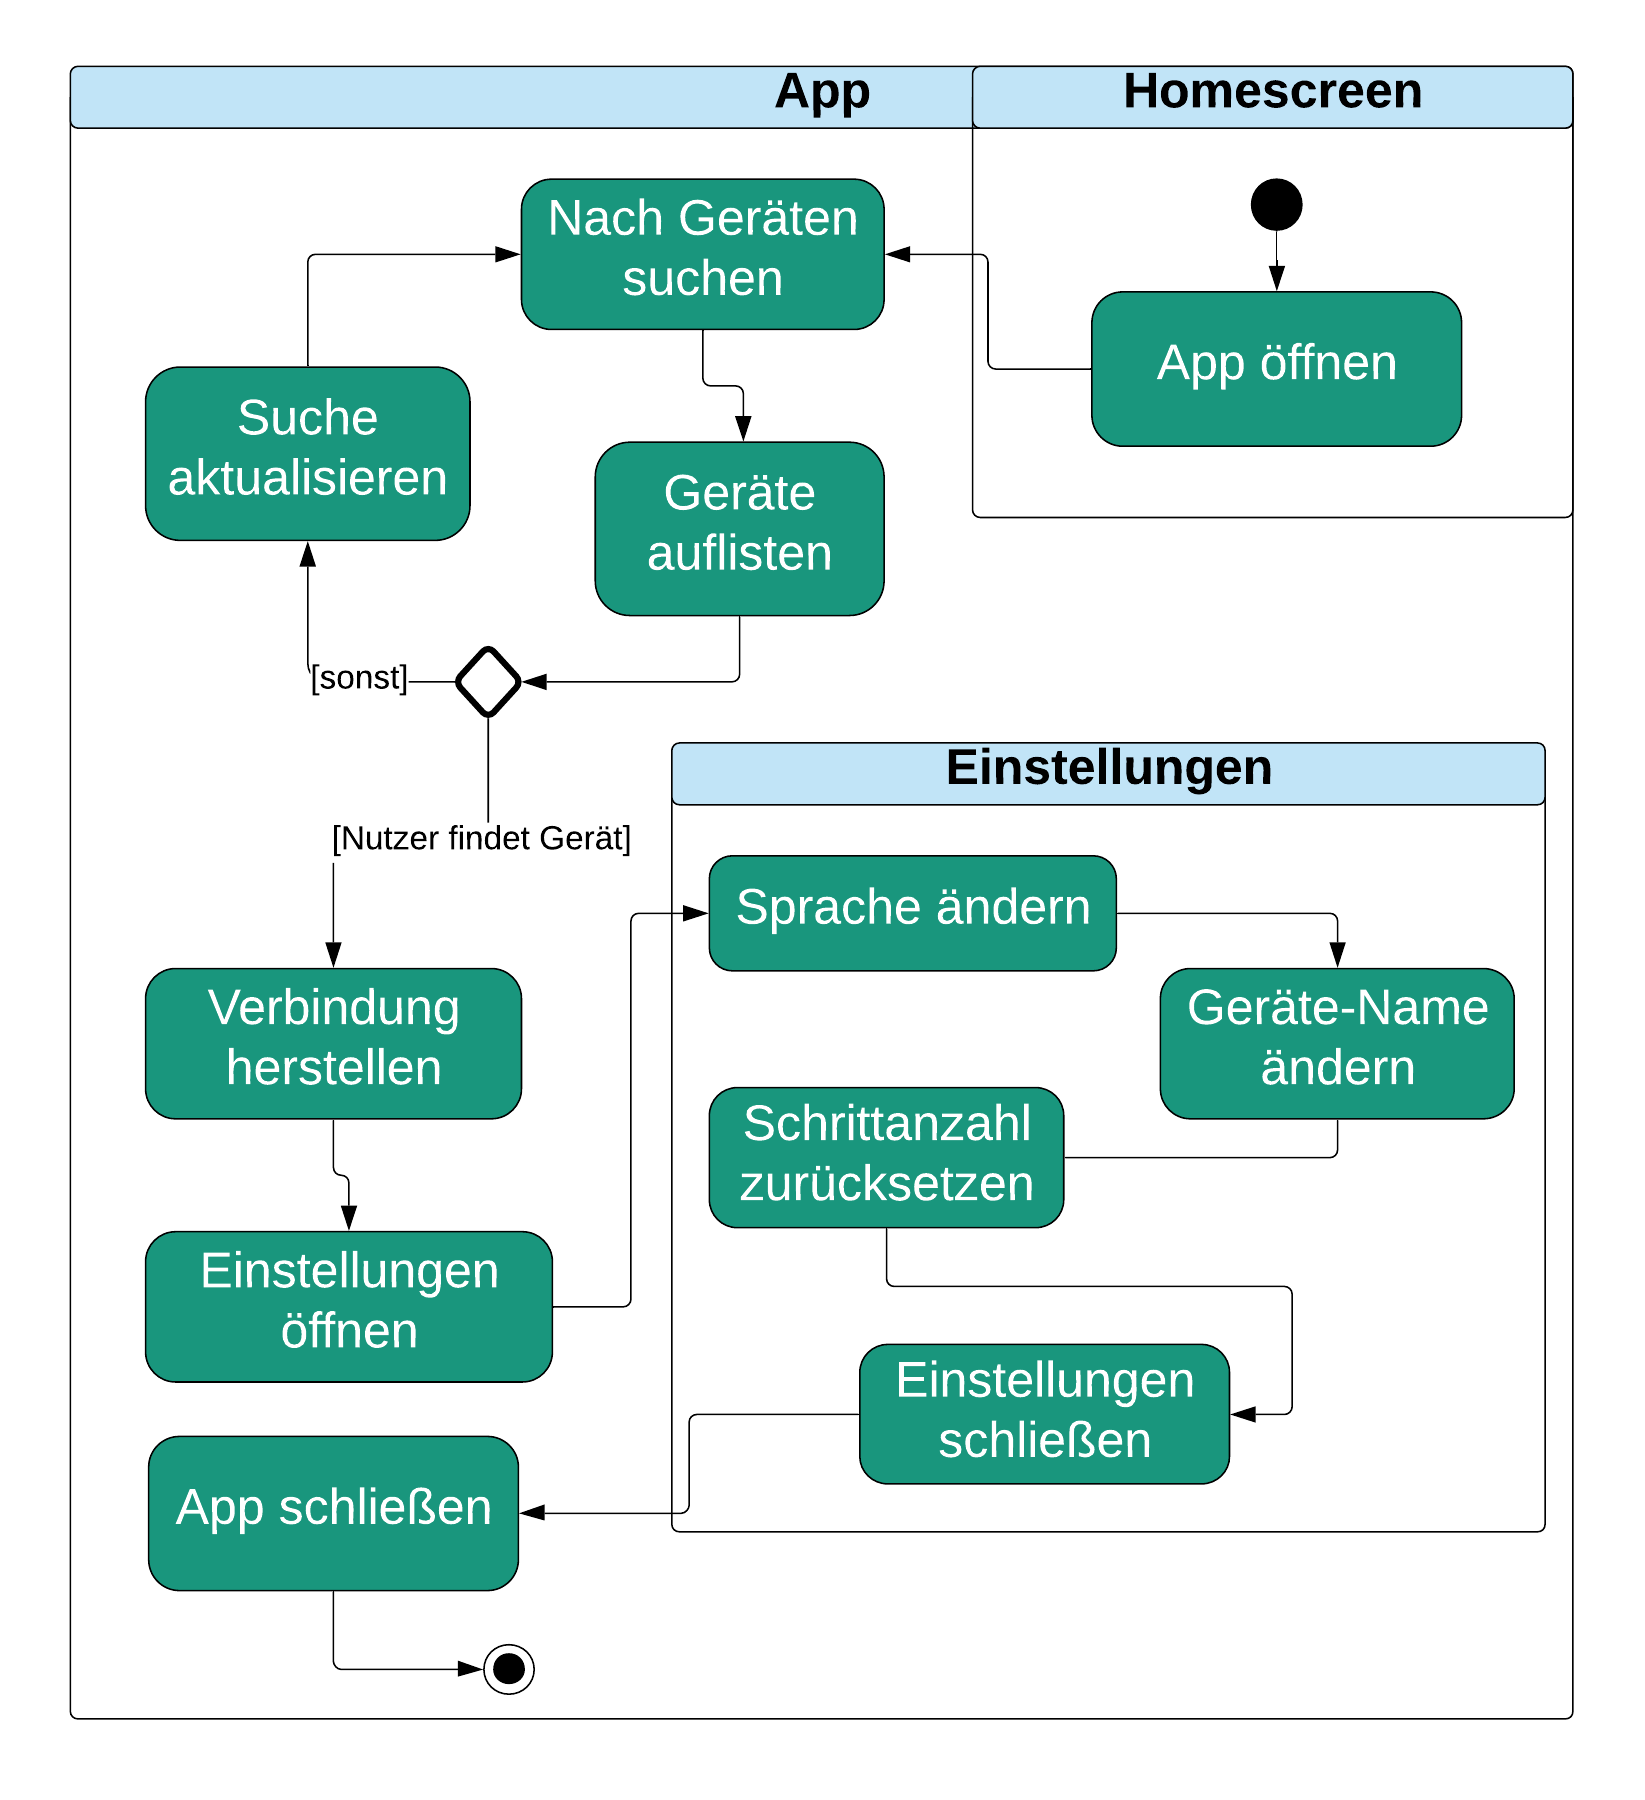
\includegraphics[page=1,width=400pt,keepaspectratio]{../graphics/UML/Konfiguration_der_Einstellungen.png}
			Hier testet der \Gls{user} die Funktionalitäten der Einstellungen (\hyperref[sec:konfigS]{Szenario})
		\subsubsection{App im Hintergrund laufen lassen}
		\label{sec:hintergrund}
			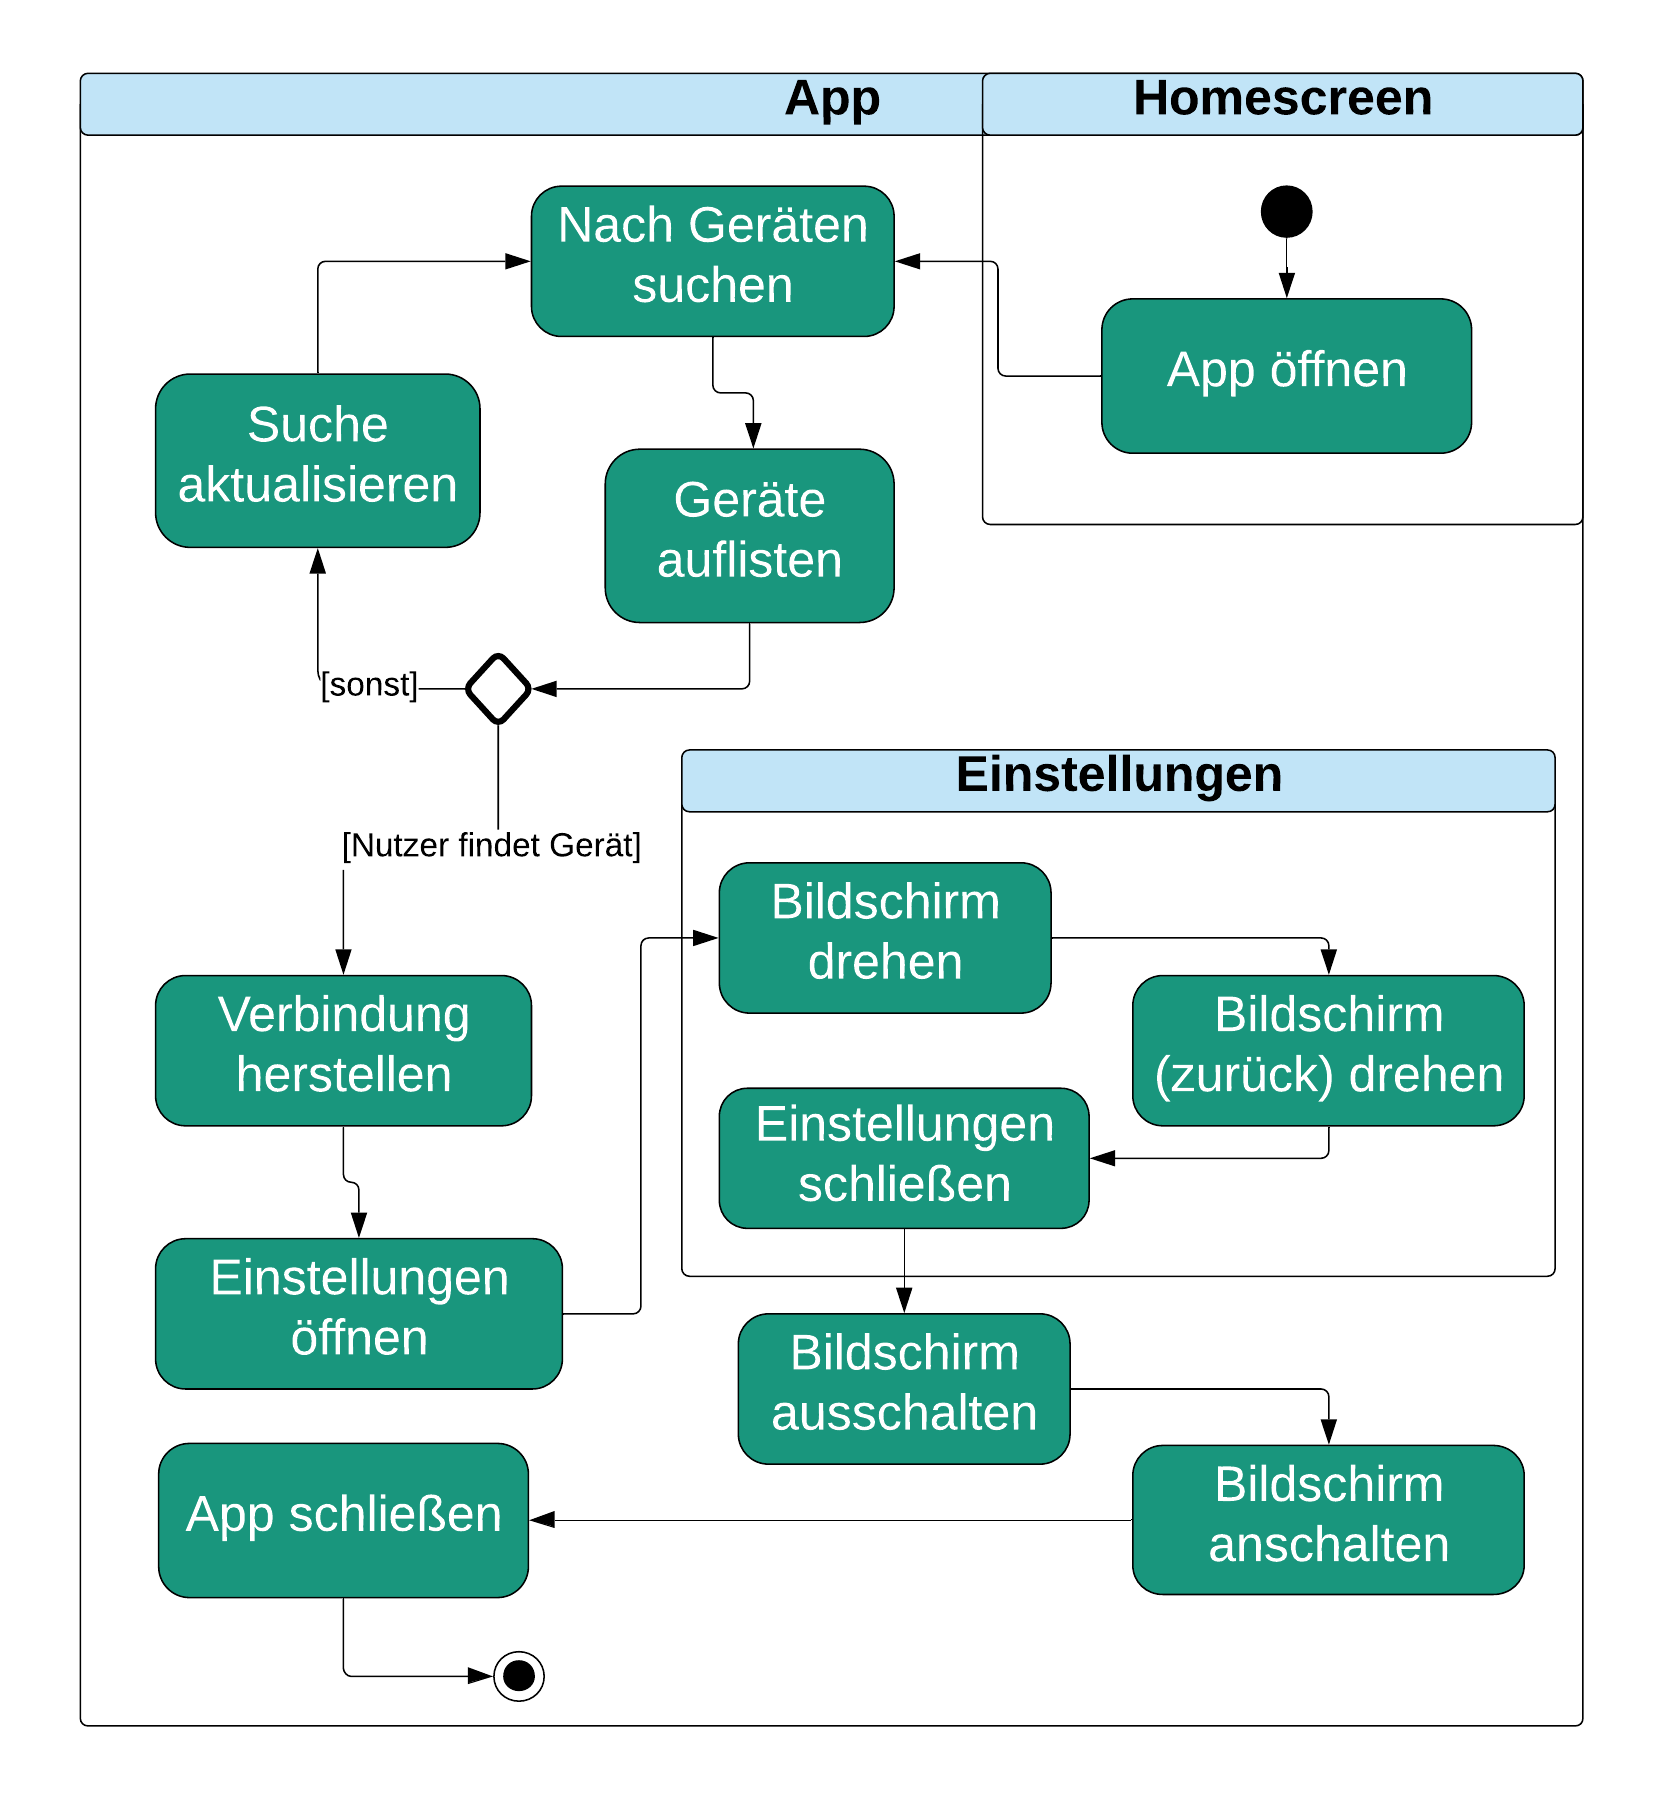
\includegraphics[page=1,width=400pt,keepaspectratio]{../graphics/UML/App_im_Hintergrund_laufen_lassen.png}
			Hier testet der \Gls{user} ob die App unter Einfluss von Funktionen des Smartphones noch korrekt ausgeführt wird (\hyperref[sec:hintergrundS]{Szenario})
		\subsubsection{Spotify einbinden}
		\label{sec:spotify}
			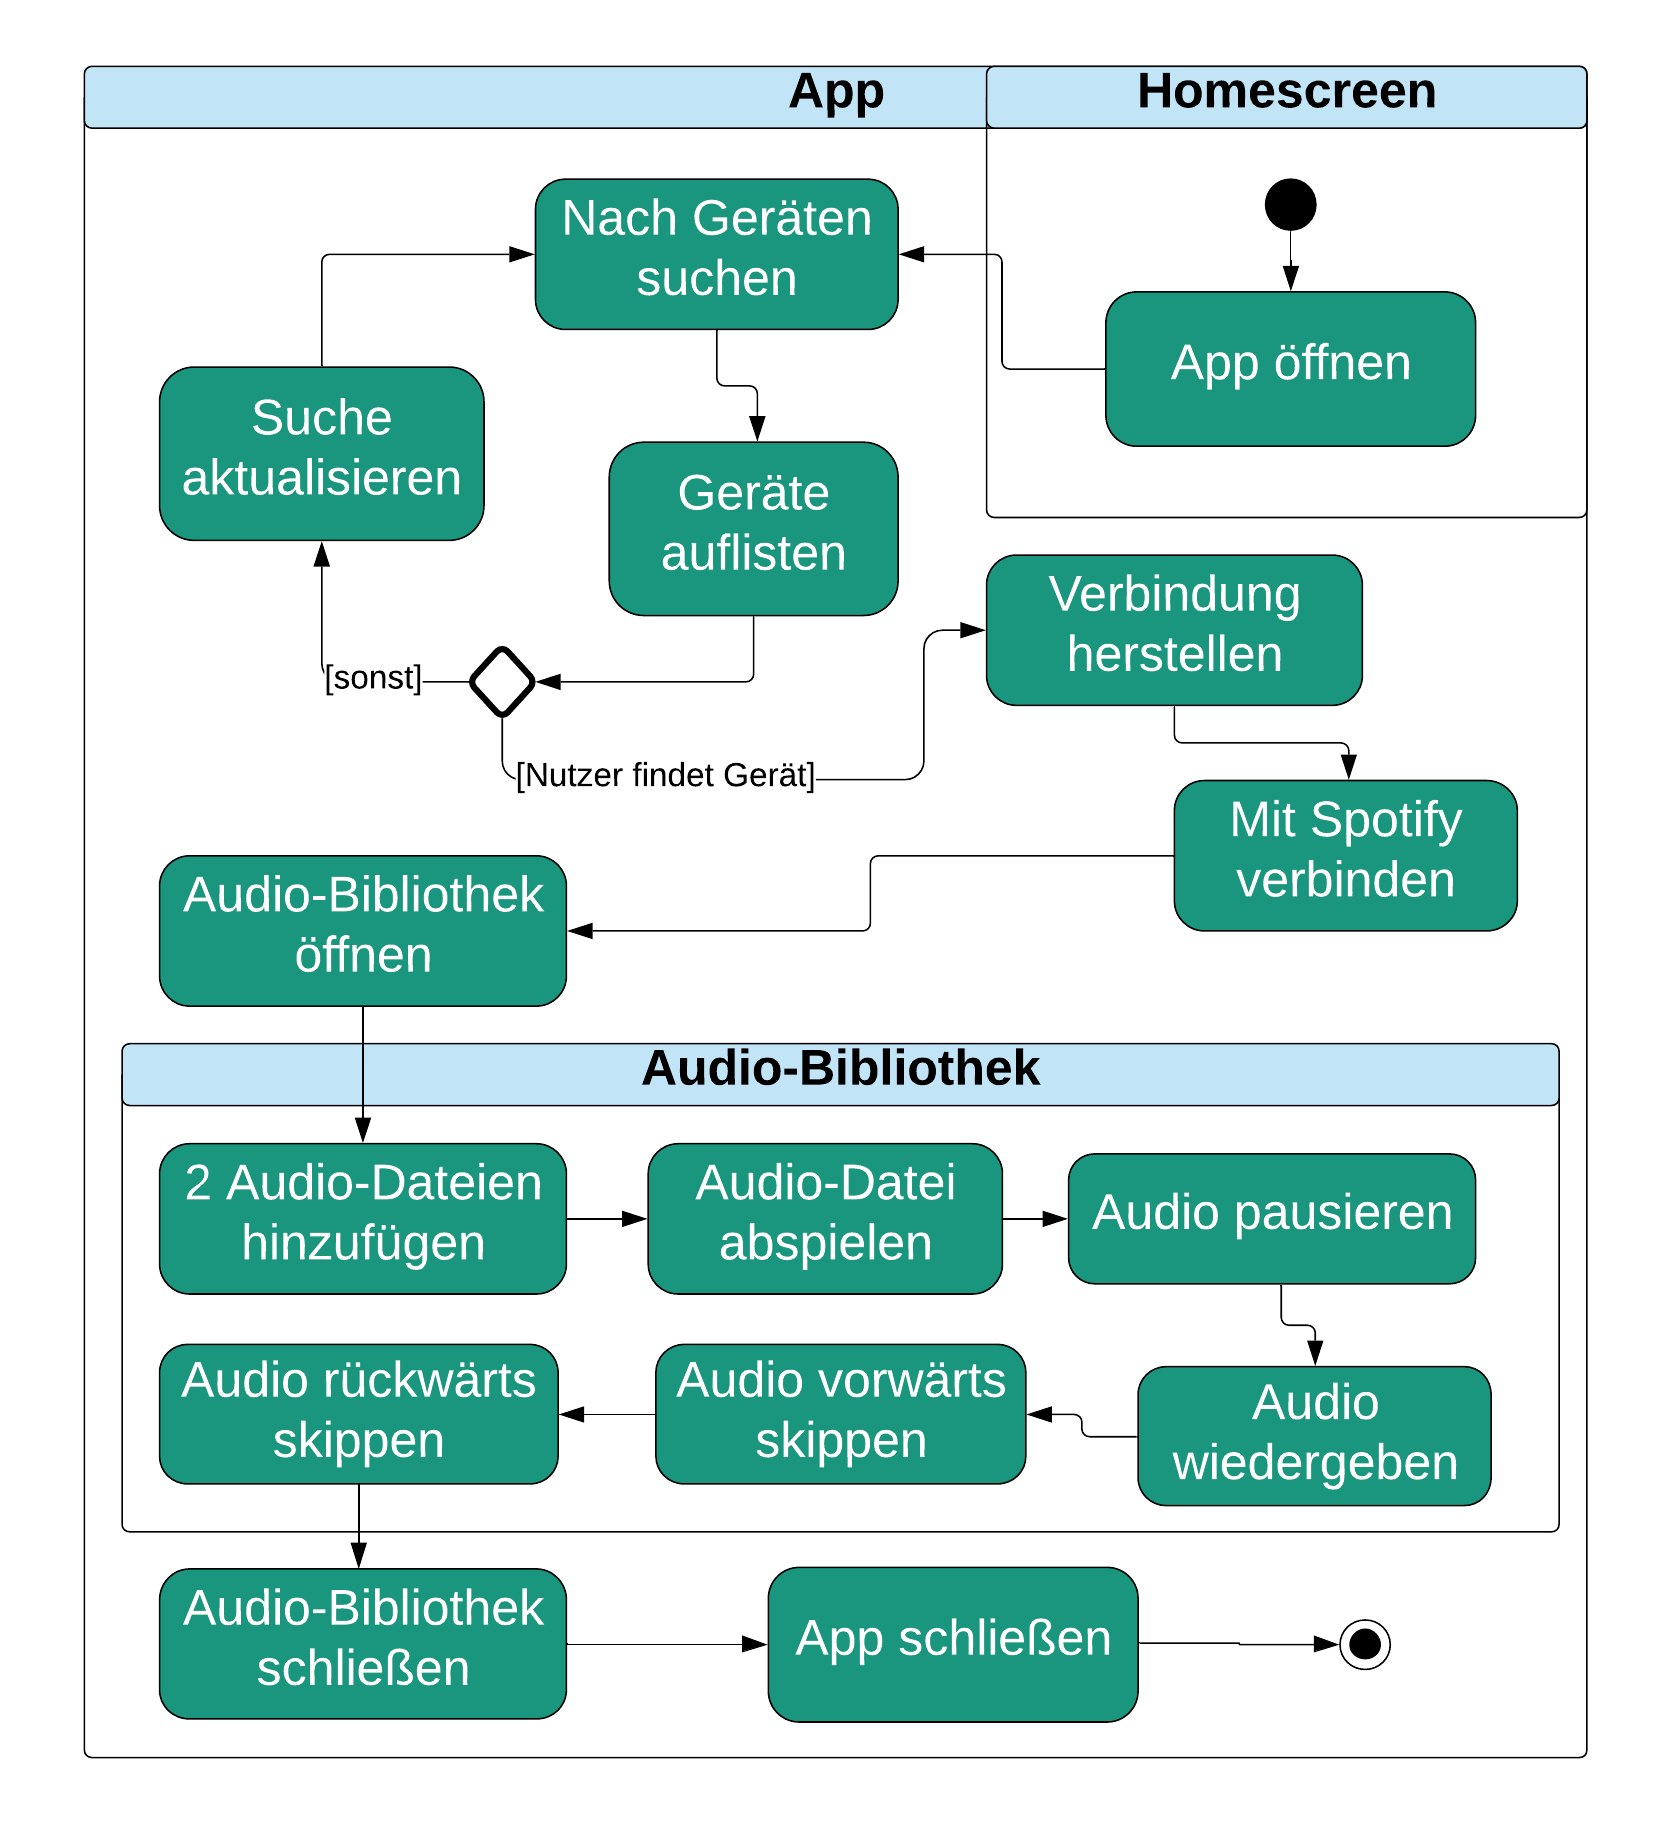
\includegraphics[page=1,width=400pt,keepaspectratio]{../graphics/UML/Spotify_einbinden.png}
			Hier testet der \Gls{user} verschiedene Funktionalitäten mit Einbindung von Spotify (\hyperref[sec:spotifyS]{Szenario})
	\subsection{Benutzerschnittstelle}
		\vspace{10mm}
		\begin{Parallel}[c]{0.4\textwidth}{0.4\textwidth}
			\ParallelLText{\noindent
				\begin{large}
					\view{10} Startbildschirm\newline
				\end{large}
				\par\noindent
				\fbox{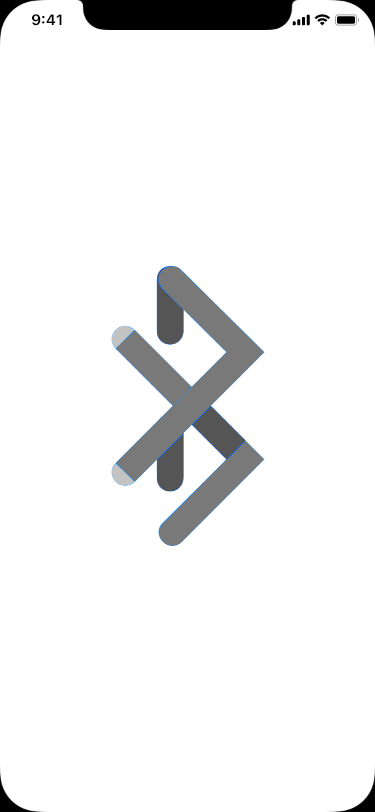
\includegraphics[width=200pt, keepaspectratio]{../graphics/GUI/Startbildschirm.png}}
				Nach Starten der \Gls{app} öffnet sich diese \Gls{view}. Ein Klick auf das \Gls{bt}-Logo startet die Suche nach Geräten.
			}
			\ParallelRText{\noindent
				\begin{large}
					\view{11} Startbildschirm\newline
				\end{large}
				\par\noindent
				\fbox{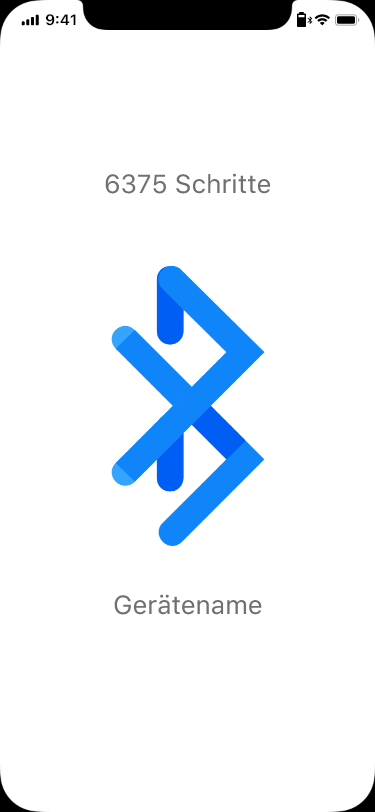
\includegraphics[width=200pt, keepaspectratio]{../graphics/GUI/Startbildschirmconnected.png}}
				Wenn die \Gls{earable}s verbunden sind wird das \Gls{bt}-Logo blau. Klicken trennt jetzt die Verbindung.
			}
		\end{Parallel}
		\vspace{10mm}
		\begin{Parallel}[c]{0.4\textwidth}{0.4\textwidth}
			\ParallelLText{\noindent
				\begin{large}
					\view{20} Verbinden\newline
				\end{large}
				\par\noindent
				\fbox{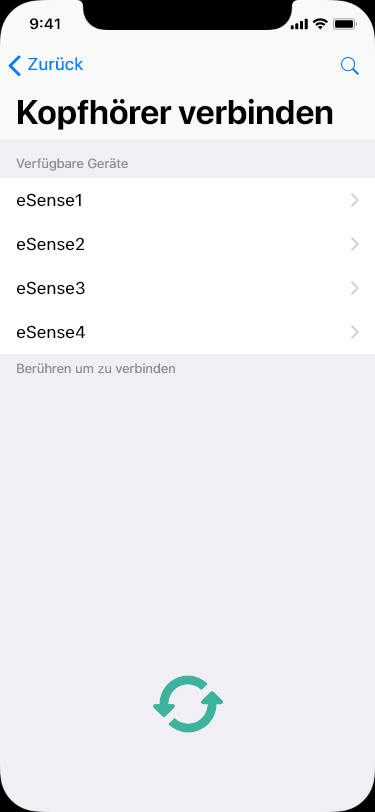
\includegraphics[width=200pt, keepaspectratio]{../graphics/GUI/Verbinden.png}}
				Ein Klick auf eines der angezeigten Geräte stellt eine Verbindung mit den entsprechenden \Gls{earable}s her.
			}
			\ParallelRText{\noindent
				\begin{large}
					\view{30} Modus-Manager\newline
				\end{large}
				\par\noindent
				\fbox{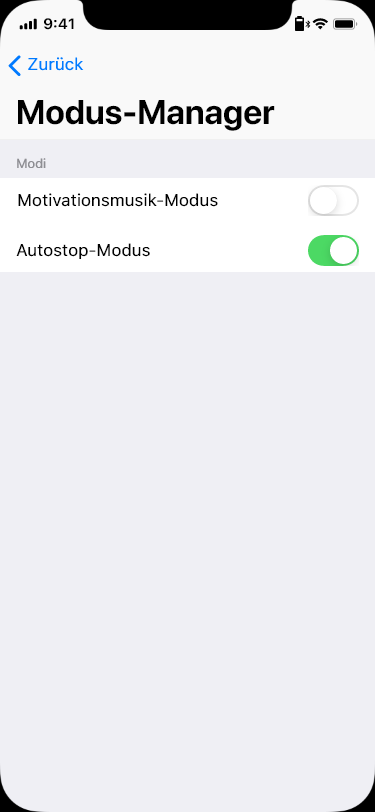
\includegraphics[width=200pt, keepaspectratio]{../graphics/GUI/Modus.png}}
				Im Modus-Manager kann man einzelne Modi an- oder ausschalten.
			}
		\end{Parallel}
		\begin{Parallel}[c]{0.4\textwidth}{0.4\textwidth}
			\ParallelLText{\noindent
				\begin{large}
					\view{40} Einstellungen\newline
				\end{large}
				\par\noindent
				\fbox{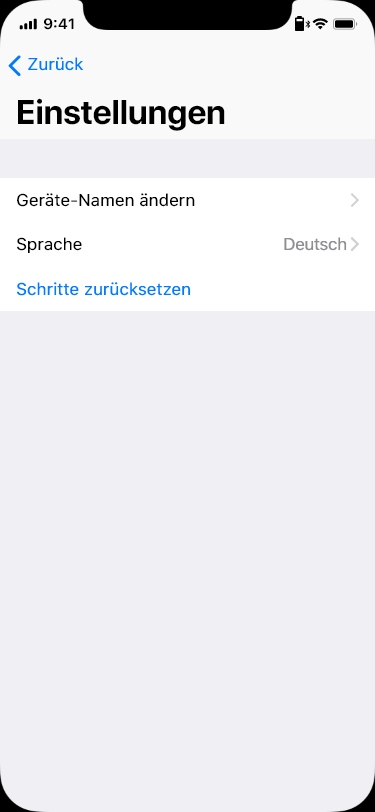
\includegraphics[width=200pt, keepaspectratio]{../graphics/GUI/Einstellungen.png}}
				In den Einstellungen kann man die \Gls{app} konfigurieren.
			}
			\ParallelRText{\noindent
				\begin{large}
					\view{50} Audio-Player\newline
				\end{large}
				\par\noindent
				\fbox{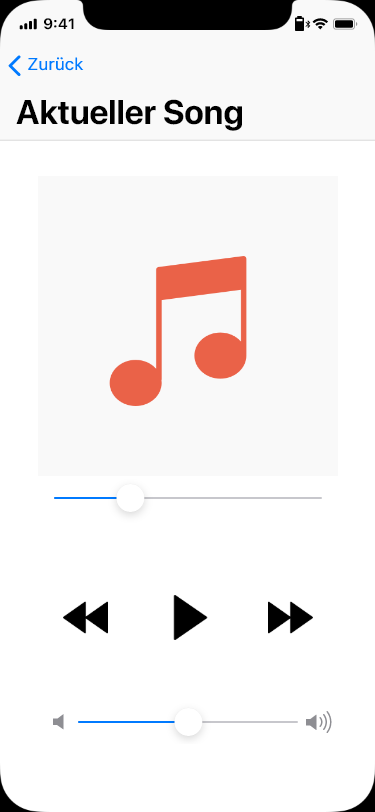
\includegraphics[width=200pt, keepaspectratio]{../graphics/GUI/Musikplayer.png}}
				Im aktiven Betrieb wird die Audio-Player-\Gls{view} angezeigt.
			}
		\end{Parallel}
		\begin{Parallel}[c]{0.4\textwidth}{0.4\textwidth}
			\ParallelLText{\noindent
				\begin{large}
					\view{60} Audio-Bibliothek\newline
				\end{large}
				\par\noindent
				\fbox{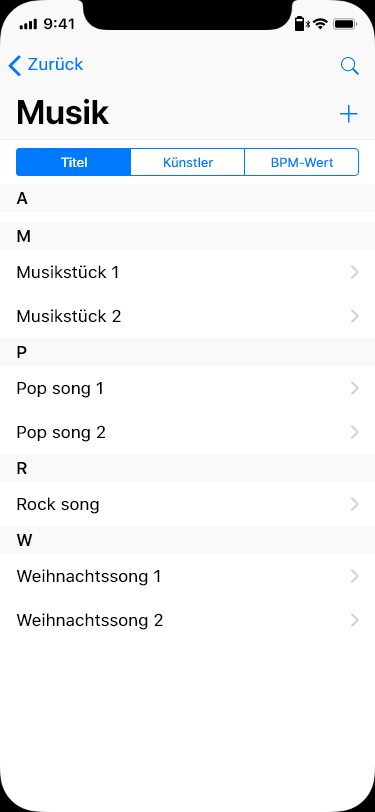
\includegraphics[width=200pt, keepaspectratio]{../graphics/GUI/Bibliothek.png}}
				In der \Gls{audiolib} kann man \Gls{audiofile}en hinzufügen
			}
		\end{Parallel}

		\newpage

\end{document}
